\chapter{Approaches to Accessing the APRS Network}
In the world of APRS, there are many solutions that hams take advantage in order to utilize the network. Some they find and make work, some they purchase to use exclusively for APRS, and some go through the trouble of building their own solutions. This chapter explains some of the common systems used on the APRS network, primarily those that can be used for receiving, starting with terminal node controllers and progressing to software based demodulation.

\section{Terminal Node Controllers}
Currently there are many systems that will demodulate these Bell 202 encoded APRS packets. The original hardware used for this communication style was dedicated modems similar to dial-up 56k modems that did the encoding and decoding. These modems were connected directly to the radio and the would decode the signal that the radio received as well as sending audio to the radio to transmit. Similarly, the terminal node controller (TNC), a specialized modem used in APRS operation, would let the radio know by signalling the radio to transmit when it had data to send out\,\cite{Wolfgang2005}. A reminder of the age of the technologies that are being used for the data transport of APRS, packet radio originated in the 1980s as TNCs became affordable\,\cite{Helms1992}. This means that this technology is over 30 years old at the time of writing in the year 2016.

With a radio and a TNC, amateur packet stations and digipeaters (digital packet repeaters) are possible\,\cite{Group2012,Wiki2012}. Digipeaters are an essential part of the ham packet network, but many users wish to report their GPS position onto the APRS network instead of just relaying traffic for other stations. In order to accomplish this, a GPS receiver is required. Now, stations can take the data from their GPS receiver and put it in the payload of the APRS packet and transmit the GPS reported position onto the network. One other common use of a TNC is an Internet attached digipeater, usually though the use of a computer, that would allow the data to be posted to the APRS-IS servers\,\cite{Community2015}. To give an example of some of the TNCs available, those within the testing testing scope of this project will be listed. There are a total of eight TNCs - six unique models - whose decoding results are compared to the software approaches. These modems included two Kantronics KAM Plus, a Kantronics KAM, an MFJ-1278, two AEA PK-88, a PK-232, and a PK-232MBX. An example image of what a TNC looks like can be seen in Figure \ref{kantronicsKamPlus}.

\begin{figure}
  \centering
	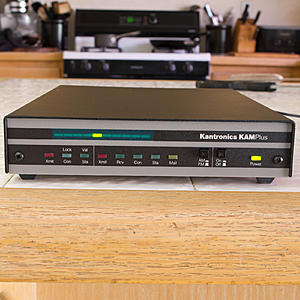
\includegraphics[width=0.75\linewidth]{images/Kantronics-KAM-Plus.jpg} 
	\caption{Image of the Kantronics KAM Plus TNC\,\cite{KK6RF}}
   \label{kantronicsKamPlus}
\end{figure}

\section{Specialized APRS Hardware}
Many people know exactly what they would like to do with APRS and exactly what traffic they want to contribute to the APRS network. So, instead of purchasing an expensive Multi-mode TNC, companies are making these dedicated APRS items available to consumers for a fraction of the price. In addition to making this hardware available, the producers support the hardware and make pretty user interfaces for the users to be able to program the hardware exactly as they like and without having to invest much time into understanding how different components work together. Some examples of APRS exclusive devices are Argent Data's OpenTrackers (Figure \ref{openTracker3}), Byonics' TinyTrack, and Fox Delta's Fox Track\,\cite{Miller,Byonics,Foxtrak}. These compact packages along with a radio and a GPS module perform APRS tasks at a satisfactory level for many users.

\begin{figure}
  \centering
	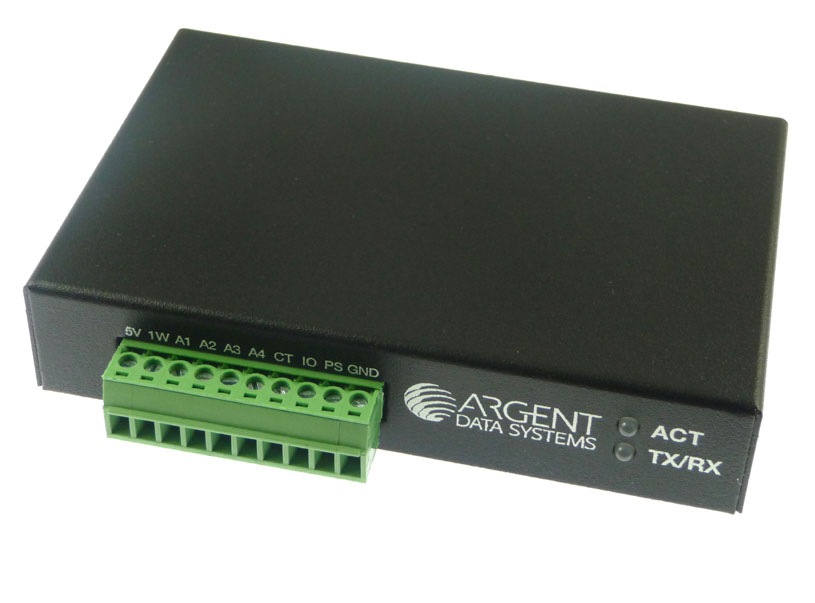
\includegraphics[width=0.75\linewidth]{images/Ot3m-termblk.jpg} 
	\caption{Image of Argent Data's OpenTracker 3.\,\cite{Data}}
   \label{openTracker3}
\end{figure}

Since the average user only wants to report positional information, these dedicated devices are simple to setup to do such tasks, but include only a simple feature set. Although these trackers contain some features, since they are all small embedded systems they cannot and do not have implemented all of the features that APRS supports. An example is the messaging service; since these devices do not have a display or a keypad, there is no way to input or display a message. Certain radio manufacturers have begun integrating the TNCs into the radios themselves to utilize the radio�s screen. The Kenwood TM-D700 series and Yaesu FTM-350 (Figure \ref{yaesuFTM350}) are examples\,\cite{Kenwood,Yaesu}.

\begin{figure}
  \centering
	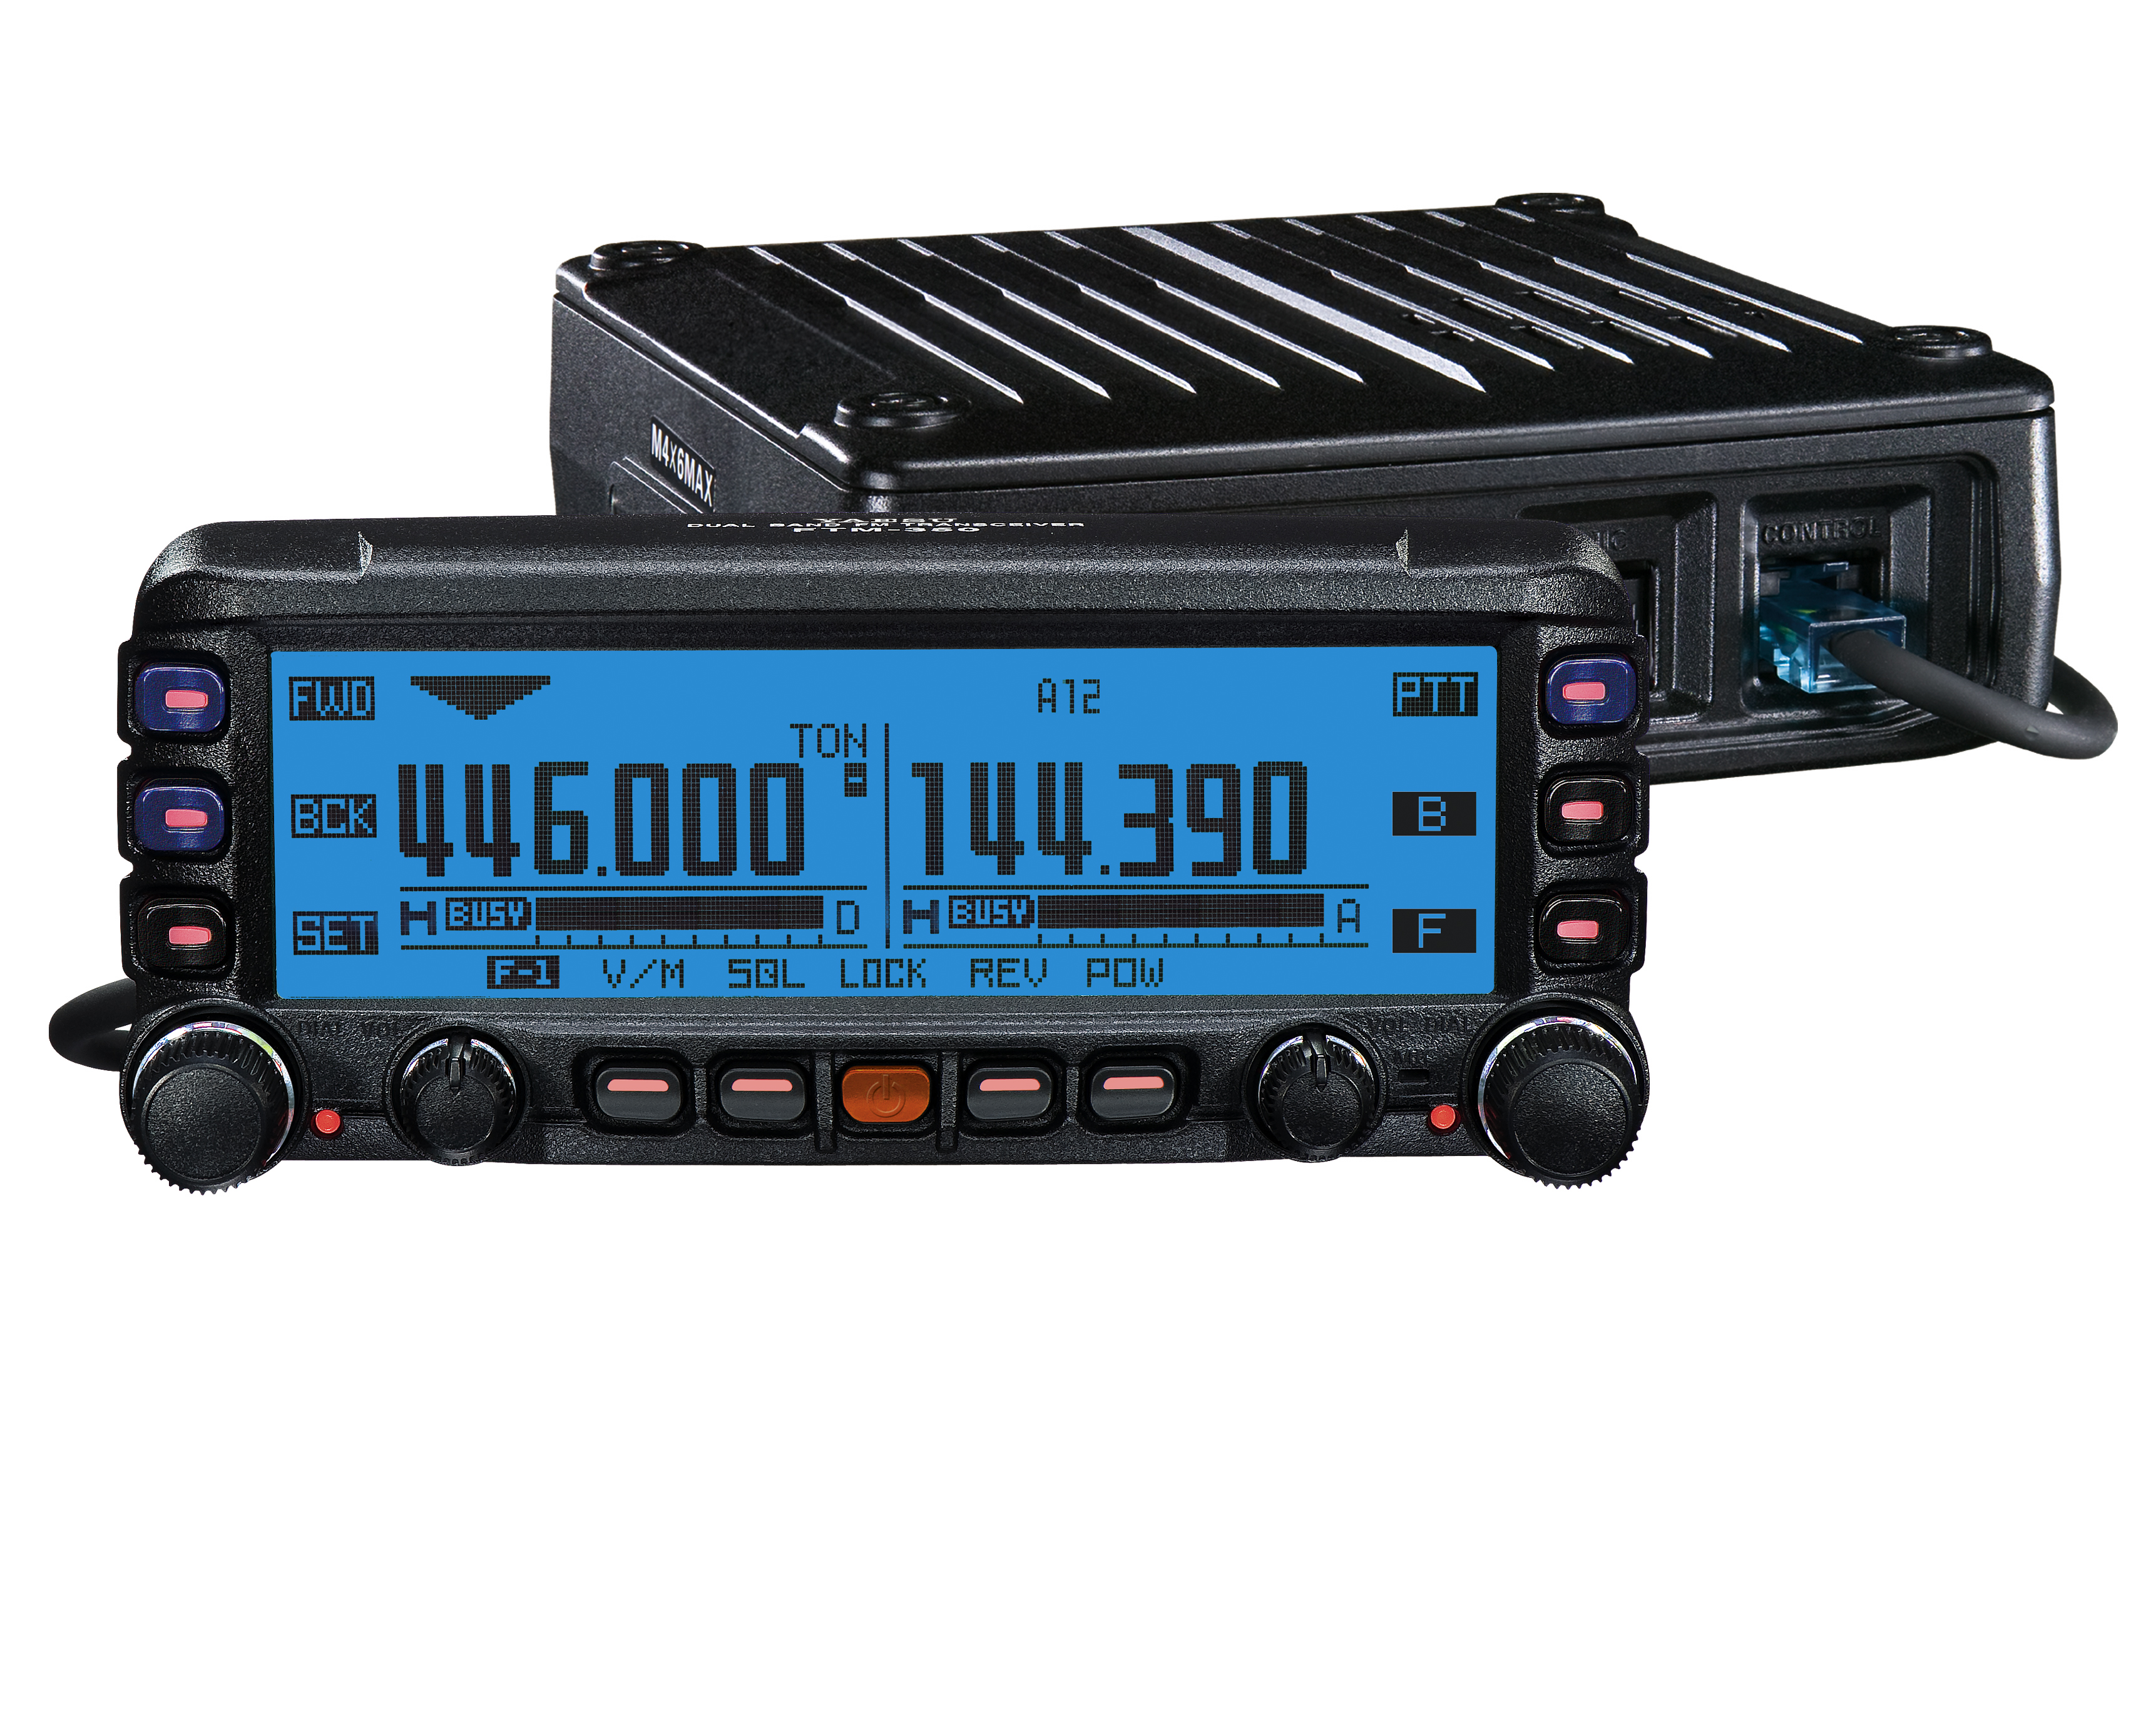
\includegraphics[width=0.75\linewidth]{images/FTM-350US_F.jpg} 
	\caption{Image of the Yaesu FTM-350 Radio which has APRS integrated.\,\cite{Yaesua}}
   \label{yaesuFTM350}
\end{figure}

However, both the options in this section and the one previous on TNCs require going out and buying special hardware in order to perform APRS. This can be expensive and cost prohibitive for some hams to be able to begin APRS operations.

\section{Software Based Demodulation}
It's fair to assume that before a ham operator becomes interested in the APRS network and sending APRS packets that they will already have a radio. So, if they already have a radio all they have to do is buy a piece of hardware that will do the modulation in order to send a packet. However, hardware costs money and before diving right in, some users might appreciate being able to try things out first. A good, cheap alternative to dedicated hardware is to use hardware that hams already have. A good choice that will fit the needs is a computer, which most hams are likely to already own. If they don't happen to own a computer, much of this argument is null and void since a computer is required to use both TNCs and to program the specialty hardware. On the computer amateurs can use software to do the modulation and demodulation, and build or buy a cheap interface to a radio, around \$15 instead of roughly \$150 for a piece of dedicated hardware.

This seems to be a route that some are taking and a demodulation scheme that this project explores in detail, but before exploring this in more detail, more information on current systems that operate in this software realm is necessary. Some examples of the software that can be used are George Rossopoylos's Packet Engine\,\cite{Rossopoylos}, Thomas Sailer's Linux Sound Modem\,\cite{Sailer1997,Sailer2000}, and Sivan Toledo's JavaAX25\,\cite{javax25github, Toledo2012a}. On a computer, even one with minimal resources, there are algorithms that are being used to demodulate the APRS packets. Again, what this project aims to investigate is what improvements can be made to the algorithms and software-based demodulation approaches in order to decode these packets in a more robust fashion and to try and get similar performance to TNCs and dedicated hardware. Based on observations in initial analyses where software was unable to decode packets, the hypothesis was made that improvements can be made to software based demodulation.

\subsection{javAX25}
Sivan Toledo's javAX25 is one method of utilizing the APRS network. Toledo's software is very comprehensive in handling the encoding, decoding, radio control, and interfacing with sound cards to allow for full use of APRS. However, in addition to just being able to utilize APRS, there is also a test application inside of this package that allows for quick and easy testing of everything in the suite - of the most interest, however, is the ability to be able to test demodulators. Although all of these features were included, the three primarily used in this project were the modulation, demodulation, and demodulator testing. Due to its comprehensiveness and ease of access online through Github, javAX25 was chosen to be the basis for this project\,\cite{javax25github}. For a complete list of features the manual can be found in the following reference, and even from the beginning the mission statement he outlines coincides with that of this research\,\cite{Toledo2012a}.

Toledo did some benchmarking of his software and found that running two demodulators in parallel provided the best results. The demodulators were exactly the same; the only difference was that one was processing data after a bandpass filter that was just centered around the two frequencies of interest, and the other had a bandpass filter that in additionally applied 6dB of attenuation at 1200Hz\,\cite{Toledo2012}. Being published in 2012, this is the newest reference in this paper on the subject of AX.25, which provided additional incentive to use this project for this research. As added verification of making the correct decision of what software to use, a very popular Android APRS application written by Georg Lukas uses javAX25 by a direct import\,\cite{APRSdroid}.